\documentclass[a4paper,11pt,openany]{kth-mag}
\usepackage[T1]{fontenc}
\usepackage{textcomp}
\usepackage{lmodern}
\usepackage{amsmath}
\usepackage[utf8]{inputenc}
\usepackage[swedish,english]{babel}
\usepackage{csquotes}
\usepackage{csvsimple}
\usepackage{hyperref}
% Default fixed font does not support bold face
\DeclareFixedFont{\ttb}{T1}{txtt}{bx}{n}{12} % for bold
\DeclareFixedFont{\ttm}{T1}{txtt}{m}{n}{12}  % for normal

% Custom colors
\usepackage{color}
\definecolor{deepblue}{rgb}{0,0,0.5}
\definecolor{deepred}{rgb}{0.6,0,0}
\definecolor{deepgreen}{rgb}{0,0.5,0}

\usepackage{listings}

% Python style for highlighting
\newcommand\pythonstyle{\lstset{
language=Python,
basicstyle=\ttm,
otherkeywords={self},             % Add keywords here
keywordstyle=\ttb\color{deepblue},
emph={MyClass,__init__},          % Custom highlighting
emphstyle=\ttb\color{deepred},    % Custom highlighting style
stringstyle=\color{deepgreen},
frame=tb,                         % Any extra options here
showstringspaces=false            % 
}}


% Python environment
\lstnewenvironment{python}[1][]
{
\pythonstyle
\lstset{#1}
}
{}

% Python for external files
\newcommand\pythonexternal[2][]{{
\pythonstyle
\lstinputlisting[#1]{#2}}}

% Python for inline
\newcommand\pythoninline[1]{{\pythonstyle\lstinline!#1!}}

\usepackage{modifications}
\usepackage[                    % References
        backend=biber
    ]{biblatex}
    \addbibresource{references.bib}
\usepackage{standalone}
\def\code#1{\texttt{#1}}

\title{Optimizing parallel transformation of data sets with processing order constraints in Python}

\subtitle{Duis autem vel eum iruire dolor in hendrerit in
          vulputate velit esse molestie consequat, vel illum
          dolore eu feugiat null}
\foreigntitle{Lorem ipsum dolor sit amet, sed diam nonummy nibh eui
              mod tincidunt ut laoreet dol}
\author{Dexter Gramfors}
\date{June 2016}
\blurb{Master's Thesis at NADA\\Supervisor: Stefano Markidis\\Examiner: Erwin Laure}
\trita{TRITA xxx yyyy-nn}
\begin{document}
\frontmatter
\pagestyle{empty}
\removepagenumbers
\maketitle
\selectlanguage{english}
\begin{abstract}
    Financial data is often represented with rows of values, contained in a dataset. This data needs to be transformed into a common format in order for
comparison and matching to be made, which can take a long time for larger datasets.
The main goal of this master’s thesis is speeding up these transformations through parallelization using Python multiprocessing.
The datasets in question consist of several rows representing trades, and are transformed into a common format using rules known as filters. In order to devise a
parallelization strategy, the filters were analyzed in order to find ordering constraints, and the Python profiler cProfile was used to find bottlenecks
and potential parallelization points. This analysis resulted in the use of a task-based approach for the implementation, in which the transformation
was divided into an initial sequential pre-processing step, a parallel step where chunks of several trade rows were distributed among workers, and a
sequential post processing step. 

The implementation was tested by transforming four datasets of differing sizes using up to 16 workers, and execution time and memory consumption
was measured. The results for the tiny, small, medium, and large datasets showed a speedup of 0.5, 2.1, 3.8, and 4.81. They also showed linearly increasing
memory consumption for all datasets.  The test transformations were also profiled in order to understand the parallel program’s behaviour for the
different datasets. The experiments gave way to the conclusion that dataset size heavily influences the speedup, partly because of the fact that
the sequential parts become less significant.  In addition, the large memory increase for larger amount of workers is noted as a major downside of
multiprocessing when using caching mechanisms, as data is duplicated instead of shared.

This thesis shows that it is possible to speed up the dataset transformations using chunks of rows as tasks, though the speedup is relatively low.

\end{abstract}
\clearpage
\begin{foreignabstract}{swedish}
    Finansiell data representeras ofta med rader av värden, samlade i en datamängd. Denna data måste transformeras
till ett standardformat för att möjliggöra jämförelser och matchning. Detta kan ta lång tid för stora
datamängder. Huvudmålet för detta examensarbete är att snabba upp dessa transformationer genom parallellisering
med hjälp av Python-modulen multiprocessing. Datamängderna omvandlas med hjälp av regler, kallade filter.
Dessa filter analyserades för att identifiera begränsningar på ordningen i vilken datamänden kan behandlas,
och därigenom finna en parallelliseringsstrategi. Python-profileraren cProfile användes även för att hitta
potentiella parallelliseringspunkter i koden. Denna analys resulterade i användandet av ett ``task''-baserat
tillvägagångssätt, där transformationen delades in i ett sekventiellt pre-processingsteg, ett parallelt steg 
där grupper av rader distribuerades ut bland arbetarprocesser, och ett sekventiellt post-processingsteg.

Implementationen testades genom transformation av fyra datamängder av olika storlekar, med upp till 16 
arbetarprocesser. Resultaten för de fyra datamängderna var en speedup på 0.5, 2.1, 3.8 respektive 4.81.
En linjär ökning i minnesanvändning uppvisades även. Experimenten resulterade i slutsatsen att
datamängdens storlek var en stor faktor i hur mycket speedup som uppvisades, delvis på grund av faktumet
att de sekventiella delarna tar upp en mindre del av programmet. Den stora minnesåtgången noterades som
en nackdel med att använda multiprocessing i kombination med cachning, på grund av duplicerad data.

Detta examensarbete visar att det är möjligt att snabba upp datamängdstransformation genom att använda
radgrupper som tasks, även om en relativt låg speedup uppvisades.

\end{foreignabstract}
\clearpage
\tableofcontents*
\clearpage
\listoffigures
\mainmatter
\pagestyle{newchap}
\chapter{Introduction}
    In this chapter, an introduction to the parallel computing problem domain and the specific problem of dataset transformation are
described in order to give the reader an initial view of what this thesis entails.

\section{Dataset transformation} \label{dataset_standardization}
In financial applications concerning trading, it is common for customers to upload datasets containing several rows describing trades, which may be in different formats.
One such application is triResolve, an application created in Python and maintained by TriOptima, where this thesis is conducted. 
In triResolve, customers resolve trade disputes in the OTC (Over-The-Counter) derivatives market,
which may arise due to for example differences in valuation methods.
To be able to resolve the trade disputes, customers upload the previously mentioned trade datasets to the service.

The datasets need to be processed in order to transform them into a standard format which makes comparisons between data from different customers possible.
In some cases, the size of the dataset is large enough that this transformation is slow. Out of the possible techniques for optimizing the transformation code,
this thesis will focus on parallelization. Since Python is the language used in triResolve, the parallelization of the existing program will be implemented using
parallel programming tools available in the language. 

When parallelizing a program, the workload is divided among multiple cores of a system, which execute the program in parallel.
For the dataset transformation problem, this means dividing the dataset, conceivably into chunks of rows, and performing the transformation of each of these chunks
on separate cores.

This thesis presents the challenges associated with this parallelization problem, and how to solve them.

%In some cases, the size of the dataset is large enough that this transformation is slow, and could conceivably be sped up through
%the use of parallelization. The sizes are aptly measured in number of rows, and range between 2 rows to about 1490000 rows. The time
%it takes to process the datasets range between 0.06 seconds and 15200 seconds 2 (4.2 hours).

%\subsection{Transformation with constraints}
The datasets are associated with a file format. The format specifies a set of rules, known as filters, which at times enforce
implicit constraints on the processing order in the file when performing the transformation. This thesis aims to identify these
constraints, which may affect how parallelizable a dataset is, and find a suitable parallelization strategy. Another aim is to identify the impact dataset size has on
any potential speedup. In addition, how using the Python \code{multiprocessing} module and its process-over-thread with message passing
approach affects implementation and performance will be investigated.

\section{Parallel computing}
In this thesis, a task-based approach is used to parallelize the dataset transformation \cite{chow_2015_pipeline_ppiaote}. A task is a single unit of computation, often represented as a function
and run on different threads or processes. Tasks are executed by the operating system's scheduler, and can be executed on different cores. When tasks are scheduled
on different cores, they are able to run at the same time, resulting in parallelism and possible speedup of a program. If there are more tasks than cores, the tasks
are scheduled using time-slicing, where tasks share cores.

\section{Hardware}
The parallelization in this thesis is conducted on a shared memory computer. In this setup, several computing units (cores) share one memory. Examples of
shared memory systems are common laptops and workstations.

%reduce the possible benefits of parallelization as they enforce
%inherently serial parts of the transformation program.  Since the size of the datasets as well as the type and number of their
%associated filters varies, it is plausible that the benefits of parallelization will differ significantly between different datasets.
%An overhead is associated with creating new threads or processes.  This overhead is increased in Python as the data shared between processes needs to serialized.
%Therefore, it is possible that parallelization of datasets will result in slower execution in some cases. Consequently, it is
%interesting to find the combinations of dataset sizes, as well as their filters, that result in beneficial parallelization, and which do not.
%Additionally, the complex nature of the system makes the implementation of the parallelization an interesting problem.

%\section{Parallel computing}
%The subject of parallel computing is one that has become highly relevant in recent years.
%Moore's law, the observed pattern that the number of transistors in a dense integrated circuit doubles approximately every two
%years \cite{moore_1998_cramming_cmcoic},
%has lost its relevance. The increased processor clock speed that the doubling in processors implies is no longer present because of
%overheating issues \cite[p. 1]{herlihy_2012_art_taomprr}. Because of this, manufacturers of processors now have
%largely turned to \emph{multicore} processors. In a multicore architecture, several cores which work as individual processors execute
%code simultaneously. Using this type of architecture to work on a single task to increase performance is known as \emph{parallelism}.

%Efforts to exploit parallelism automatically from a program have been made; however, the benefits of these have reached their
%limit \cite[p. 7-12]{mccool_2012_structured_spppfec}. In order to fully utilize the increase in performance that multicore
%architectures promise, programmers today must instead turn to explicit parallel programming.

%Python is one of world's most popular programming languages \cite{krill_2015_python_psnhilp}. It is used extensively both at schools and
%in the industry, and its benefits include expressiveness, portability, and the fact that it is easy to learn. Python has support for
%parallel programming, although it has caveats and overheads associated with a concurrency-hampering mechanism called the
%\emph{Global Interpreter Lock} \cite{beazley_150745UTC_introduction_aitpc}.

%This thesis concerns a combination of the areas mentioned above: parallel computing using Python.

%\section{Dataset transfromation} \label{trioptima}
%The thesis is conducted at TriOptima, a company that provides different services for the OTC derivatives market.
%In one of TriOptima's services, customers upload datasets representing trades.
%OTC derivatives concern trading directly between two parties, and the customers include large banks. TriOptima’s services
%include portfolio compression, reconciliation, dispute resolution, and risk management. The services deal with substantial
%amounts of data, and face challenges such as high security demands, availability requirements, and speed optimization
%for data transformations and risk calculations. In their reconciliation and dispute resolution service,

\section{Motivation}
The motivation of this thesis is to answer the following questions.

\emph{Given the size of a dataset and its set of filters, is it possible to determine 
if parallelization of the data transformation using Python will be beneficial or not?}

The thesis question gives rise to the following subquestions:
\begin{itemize}
    \item What is the best approach for parallelizing code in Python in order to minimize data races and maintain performance?
    \item How should the parallel performance be measured?
    \item What kind of data dependencies exist and how do they affect parallelization?
    \item What kind of overhead does parallelization introduce?
\end{itemize}

\section{Objectives}
The objectives of this thesis are to:
\begin{itemize}
    \item Analyze parallelizability of dataset file formats.
    \item Use a Python profiler to analyze \code{multiprocessing} performance for dataset transformation.
    \item Implement a working parallelization of the dataset transformation program, for the applicable datasets.
    \item Evaluate the parallel performance of transformation of different datasets by measuring execution time, speedup, and memory consumption.
\end{itemize}
%The objective of this thesis is to answer the questions stated above using a literature study and by implementing a working parallelization
%of the existing dataset processing program, subsequently analysing transformations of several datasets in order to draw conclusions about performance.

\section{Contribution}
This thesis focuses on parallelization analysis of a file format rather than the more conventional method of analyzing source code. Additionally,
it shows how Python can be effectively used for parallelization in a complex system not built for parallelization from the start. The fact that
the parallelized system relies on database operations and, consequently, I/O is another aspect of the thesis that may interest other researchers
in the field of parallel programming. Similar projects can use the conclusions of this thesis as a foundation when creating a parallelization strategy.

\chapter{Related work}
    \section{Parallelization of algorithms using python}

Ahmad et al. \cite{ahmad_2015_efficient_epoppwossm} parallelize path planning algorithms such as Dijkstra's algorithm using C/C++ and
Python in order to compare the results and evaluate each language's suitability for parallel computing. For the Python implementation,
both the \code{multiprocessing} and \code{threading} packages are used. The authors identify Python as the preferable choice 
in application development, due to its safe nature in comparison to C and C++. The implementation using the \code{threading}
module resulted in no speedup over the sequential implementation. Parallelization using the \code{multithreading} module resulted
in a speedup of 2.5x for sparse graphs, and a speedup of 6.5x for dense graphs. The overhead introduced by the interpreted nature
of Python, as well as the extra costs associated with Python multiprocessing, was evident as the C/C++ implementations showed both
better performance and better scalability. The slowdowns for sparse graph of Python compared to C/C++ ranged between
20x to 700x depending on the graphs.
However, the authors note that the parallel Python implementation exhibits scalability in comparison to its sequential implementation.
The experiments were conducted on a machine with 4 cores with 2-way hyperthreading.

Cai et al. \cite{cai_2005_performance_otpotpplfsapsc} note that Python is suitable for scientific programming thanks to its richness and
power, as well as its interfacing capabilities with legacy software written in other languages. Among other experiments on Python
efficiency in scientific computing, its parallel capabilities are investigated. The Python MPI package \code{Pypar} is used for
the parallelization, using typical MPI operations such as send and receive. The calculations, such as wave simulations, 
are made with the help of the \code{numpy} package for increased efficiency. The authors conclude that while communication 
introduces overhead, Python is sufficiently efficient for scientific parallel computing.

Singh et al. \cite{singh_2013_parallel_padpwprfmm} present Python as a fitting language for parallel computing, and use the
\code{multiprocessing} module as well as the standalone \code{Parallel Python} package in their experiments. Because of the
communication overhead in Python, the study focuses on embarrassingly parallel problems where little communication is needed.
Different means of parallelization are
compared: the Pool/Map approach, the Process/Queue approach, and the Parallel Python approach. 
In the Pool/Map approach, the simple functions of \code{multiprocessing.Pool} are used to specify a number of processes, a data
set, and the function to be executed with each element in the dataset as a parameter. In the Process/Queue approach, a
\code{multiprocessing.Queue} is spawned and filled with chunks of data. Several \code{multiprocessing.Process} objects are then
spawned, which all share the queue and get data to operate on from it while it is not empty. Another shared queue is used for
collecting the results. In the Parallel Python approach, the \code{Parallel Python} abstraction \emph{job server}
is used to submit tasks for each data chunk. The tasks are automatically executed in parallel by the job server, and the results
are collected when they have finished.  The results in general show significant time savings even though the approaches taken are relatively straightforward.
The best performance is achieved when the number of processes is equal to the number of physical cores on the computer.
The Process/Queue is shown to perform better than both Pool/Map and parallel Python. This comes at the cost of a slightly less
straightforward implementation. The impact of load balancing and chunk size is also discussed, with the conclusion that work load
should be evenly distributed among cores as computation is limited by the core that takes the longest to finish.

Rey et al. \cite{rey_2013_parallel_pocmcip} compare \code{multiprocessing} and \code{Parallel Python} with the GPU-based parallel
module \code{PyOpenCI} when attempting to parallelize portions of the spatial analysis library PySAL. In particular, different
versions of the Fisher-Jenks algorithm for classification are compared. For the smallest sample sizes, the overhead of the
different parallel implementations produce slower code, but as the sample sizes grow larger the speedup grows relatively quickly.
For the largest of the sample sizes, the speedup curve generally flattens out; the authors state this as counter-intuitive and
express an interest in investigating this further. In general, the CPU-based modules \code{multiprocessing} and \code{Parallel Python}
perform better than the GPU-based PyOpenCI. The \code{multiprocessing} module produced similar or better results than the
\code{Parallel Python} module.
While the parallel versions of the algorithm perform better, the bigger implementation effort associated with it is noted.

In the work above, the code that is parallelized is CPU bound. This differs from this thesis, as a large portion of the
to be parallelized program is I/O bound due to database interactions. Another difference is the fact that
the parallelization analysis conducted in this thesis is mainly done on the file format level rather than at program level, like the work above.
However, the works highlight aspects of parallelization using Python that are useful in achieving the thesis objective.
These include parallelization patterns, descriptions of overhead associated with parallel programming in Python, and comparisons
between different Python modules for parallelization.

\section{Python I/O performance and general parallel benchmarking}
In their proposal for the inclusion of the \code{multiprocessing} module into the Python standard library,
Noller and Oudkerk \cite{noller_pep_p0} include several benchmarks where the \code{multiprocessing} module's performance is
compared to that of the \code{threading} module. They emphasize the fact that the benchmarks are not as applicable on platforms with slow forking
time. The benchmarks show that while naturally slower than sequential execution, \code{multiprocessing} performs better than
\code{threading} when simply spawning workers and executing an empty function. For the CPU-bound task of computing Fibonacci numbers,
\code{multiprocessing} shows significantly better result than \code{threading} (which is in fact slower than sequential code). For I/O bound
calculations, which is an application considered suitable for the \code{threading} module, the \code{multiprocessing} module is still shown to have
the best performance when 4 or more workers are used.

The benchmarks where performed using the following hardware:
\begin{itemize}
  \item 4 Core Intel Xeon CPU @ 3.00GHz
  \item 16 GB of RAM
  \item Python 2.5.2 compiled on Gentoo Linux (kernel 2.6.18.6)
  \item pyProcessing 0.52
\end{itemize}

While this work is a relatively straightforward benchmark under ideal conditions, the fact that \code{multiprocessing} shows better performance than \code{threading}
for both CPU bound and I/O bound computations contributed to the decision to use \code{multiprocessing} in this thesis.

\section{Comparisons of process abstractions}
Friborg et al. \cite{friborg_2009_three_tuiopfp} explore the use of processes, threads and greenlets in their process abstraction
library PyCSP. The authors observe the clear performance benefits of using multiprocessing over threads due to the circumvention of the GIL
that the \code{multiprocessing} module allows. Greenlets are user-level threads that execute in the same thread and are unable to utilize
several cores. On Microsoft Windows, where the fork() system call is not available, the process creation is observed as
significantly slower than on UNIX-based platforms. While serialization and communication has a negative impact on performance when
using \code{multiprocessing}, the authors state that this produces the positive side-effect of processes not being able to
modify data received from other processes.

The work above focuses on process abstractions in a library, but comes to conclusions that are helpful in this thesis; \code{multiprocessing}
has performance benefits over the other alternatives, and also introduces safety to a system thanks to less modification of data sent between
processes.

\section{Parallelization in complex systems using Python}
Binet et al. \cite{binet_2010_harnessing_hmsaiia} present a case study where parts of the ATLAS software used in
LHC (Large Hadron Collider) experiments are parallelized. Because of the complexity and sensitivity of the system,
one of the goals of the study is to minimize the code changes when implementing the parallelization. The authors highlight several
benefits of using multiple processes with IPC instead of traditional multithreading, including ease of 
implementation, explicit data sharing, and easier error recovery. The Python \code{multiprocessing} module was used to parallelize
the program, and the authors emphasize the decreased burden resulting from not having to implement explicit IPC and synchronization.
Finding the parts of the program that are embarrassingly parallel and parallelizing these is
identified as the preferred approach in order to avoid an undesirably large increase in complexity while
still producing a significant performance boost. The parallel implementation was tested by measuring the user and real time for different numbers of processes.
These measurements show a clear increase in user time because of additional overhead, but also a steady decrease in real time.

Implementing parallelization of a component of a large system without introducing excessive complexity is a goal of this thesis, similar to the work above.
The above approach to parallelization, identifying embarrassingly parallel parts of the system and focusing on these, were used in this thesis. Again, 
this thesis differs from the above by having a largely I/O bound portion and by analysing a file format for parallelizability.

\section{Summary of related work}
Common themes and conclusions in the related work presented above include:

\begin{itemize}
  \item Python is a suitable language for parallel programming.
  \item The \code{multiprocessing} module is successful in circumventing the GIL and consistently shows the same or better performance than other
    methods, even for I/O bound programs.
  \item The overhead that IPC introduces when creating parallel Python programs makes it imperative to minimize communication and
    synchronization. Consequently, embarrassingly parallel programs are preferable when using Python for parallelization.
  \item For existing larger systems, extensive parallelization may produce undesired complexity.
\end{itemize}

\chapter{Theory}
    In this chapter, theory related to multicore architecture and parallel programming is
explained in order to give the reader the foundation needed to understand these aspects of
the thesis.

\section{Definitions}
\begin{itemize}
  \item \textbf{IPC} - Interprocess communication.
  \item \textbf{MPI} - Message Passing Interface. Standardized interface for message passing between processes.
  \item \textbf{Embarrassingly parallel} - A problem that is embarrassingly parallel can easily be broken down into components that
    can be run in parallel. %Cite astro? Python hpc?
  \item \textbf{CPU bound} - Calculation where the bottleneck is the time it takes for a processor to execute it.
  \item \textbf{I/O bound} - Calculation where the bottleneck is the time it takes for some input/output call, such as file accesses
    and network operations.
  \item \textbf{Real time} - The total time it takes for a call to finish.
  \item \textbf{User time} - The time a call takes, excluding system overhead; the time the call spends in user mode.
  \item \textbf{System time} - The time in a call that is consumed by system overhead; the time the call spends in kernel mode.
  \item \textbf{DAG/Directed acyclic graph} A directed graph that contains no directed cycles.
\end{itemize}

\section{Multicore architecture}
\subsection{Processes vs threads}
While both threads and processes represent contexts in which a program is run, they have a few differences. A thread is run inside
a process, and the threads within the process share memory and state with each other and the parent
process \cite{singh_2013_parallel_padpwprfmm}. Individual processes do not share memory with each other, and any
communication between processes must be done with message passing rather than with shared memory. Consequently, communication
between threads is generally faster than between processes.
Typically, different threads can be scheduled on different cores, which is also true for different processes.

\subsection{Multicore communication and caching}
Multiple processors communicate with each other through a bus or a network \cite[p. 472-476]{herlihy_2012_art_taomprr}. Since the
means of communication between the processes is a finite resource, too much traffic may result in delays. The processors typically
have their own cache. In order to avoid unnecessary reads from the slower main memory, processors may read from another processor
that has the requested data cached. In a process called \emph{cache coherence}, shared cached values are kept up to date using one
of several protocols. The effect that these different means of communication between processors has on performance in
multiprocessor programs should not be ignored.

\section{Parallel shared memory programming}

\subsection{Data parallelism}
Data parallelism denotes code where the parallelism comes from decomposing the data and running it with the same piece of code
across several processors or computers \cite{singh_2013_parallel_padpwprfmm}. It allows scalability as number of cores and problem
sizes increase, since more parallelism can be exploited for larger datasets \cite[p. 24]{mccool_2012_structured_spppfec}.

\subsection{Task parallelism}
In task parallelism, groups of tasks that are independent are run in parallel \cite{chow_2015_pipeline_ppiaote}.
Tasks that depend on each other cannot be run in parallel, and must instead be run sequentially.
A group of tasks is embarrassingly parallel if none of the tasks in the group depend on each other.

\subsection{Scheduling}
Threads and processes are scheduled by the operating system, and the exact mechanism for choosing what to schedule when differs
between platforms and implementations \cite[p. 472]{herlihy_2012_art_taomprr}. Scheduling may imply running truly parallel
on different cores, or on the same core using time-slicing. Threads and processes may be descheduled from running temporarily for several
reasons, including issuing a time-consuming memory request.

\section{Performance models for parallel speedup}

\subsection{Amdahl's law}
Amdahl's law \cite{amdahl_2013_computer_caaal} states that:
\begin{displayquote}
The effort expended on achieving high parallel processing rates is wasted unless it is
accompanied by achievements in sequential processing rates of very nearly the same magnitude.
\end{displayquote}

Amdahl divides programs into two distinct parts: a parallelizable part and an inherently
serial part
\cite[p. 13]{herlihy_2012_art_taomprr}.
If the time it takes for a single worker (for example, a process) to complete the program is $1$, Amdahl's law says
that the speedup $S$ of the program with $n$ workers with the parallel fraction of the program $p$ is:
\begin{displaymath}
  S = \frac{1}{1 - p + \frac{p}{n}}
  \label{amdahl}
\end{displaymath}

The law has the following implication: if the number of workers is infinite, the time it takes for a program to finish is still
limited by its inherently serial fraction. This is illustrated below:

\begin{displaymath}
  \lim_{n \to \infty} \frac{1}{1 - p + \frac{p}{n}} = \frac{1}{1 - p}
  \label{amdahl_lim}
\end{displaymath}

$1-p$ is the serial fraction which clearly limits the speedup of the program even with an unlimited number of processors.

\subsection{Extensions of Amdahl's law}
Che and Nguyen expand on Amdahl's law and adapts it to modern multicore processors \cite{che_2014_amdahl_alfmmp}. They find that
more factors than the number of workers affect the performance of the parallelizable part of a program, such as if the work is
more memory bound or CPU bound. In addition, they find that with core threading (such as hyperthreading), superlinear speedup of a
program is achievable and that the parallelizable part of a program is guaranteed to also yield a sequential term due to resource
contention.

Yavits et al. come to similar conclusions \cite{yavits_2014_effect_teocasoalims}. They find that it is important to minimize the
intensity of synchronization operations even in programs that are highly parallel.

\subsection{Gustafson's law}
Gustafson's law \cite{gustafson_1988_reevaluating_ral} is a result of the observation that problem sizes often grow with the
number of processors, an assumption that Amdahl's law dismisses, keeping the problem size fixed. With this premise, a program can
be run with a larger problem size in the same time as more workers are added. This view is less pessimistic than Amdahl's law, as
it implies that the impact of the serial fraction of a program becomes less significant with many workers and a large problem
size \cite[p. 61-62]{mccool_2012_structured_spppfec}.

The speedup $S$, for $n$ workers, and $s$ and $p$ as the time spent in the serial and parallel parts in the parallel system,
respectively, is achieved by:

\begin{displaymath}
  S = n + (1-n) * s
\end{displaymath}

\subsection{Work-span model} \label{work-span}
The tasks that need to be performed in a program can be arranged to form a directed acyclic graph, where a task that
has to be completed before another precedes it in the graph. The work-span model introduces the following terms
\cite[p. 62-65]{mccool_2012_structured_spppfec}:
\begin{itemize}
  \item \textbf{Work} - The work of a program is the time it takes to complete with a single worker, and equals the total time it
    takes to complete all of the tasks. The work is denoted $T_1$.
  \item \textbf{Span} - The span of a program is the time it takes for the program to complete with an infinite number of workers.
    The span is denoted $T_\infty$.
  \item \textbf{Critical path} - The tasks that are included in the path that has the maximum number of tasks that need
    to be executed in sequence. The span is equal to the length of the critical path.
\end{itemize}

An example of a task DAG can be found in figure \ref{fig:dag_example}.

\begin{figure}[ht]
  \centering
  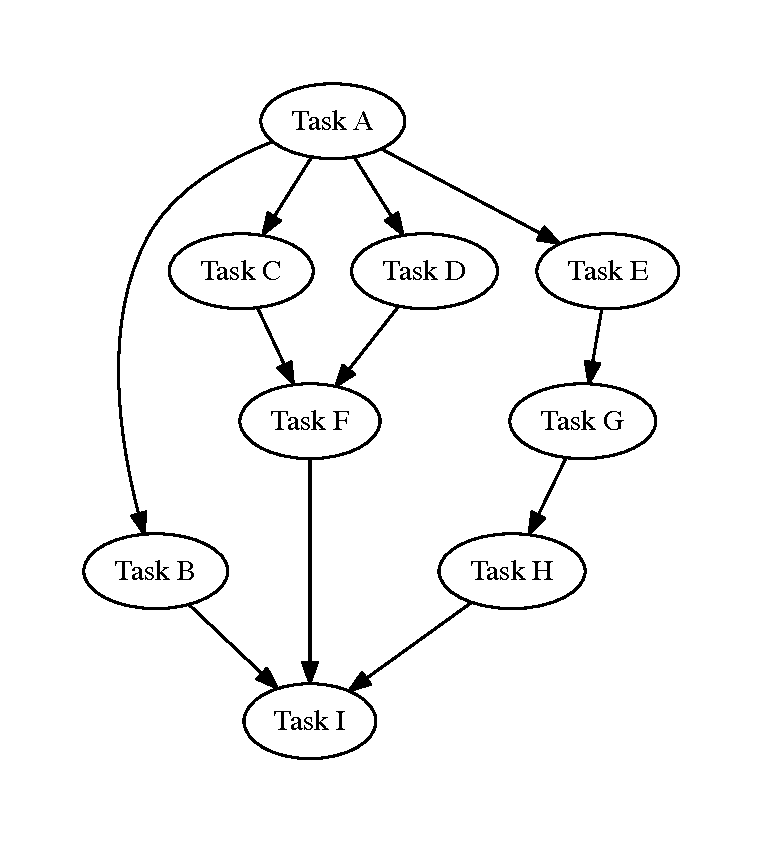
\includegraphics[width=120mm]{figures/task_dag_example.pdf}
  \caption[Example of work-span model task DAG]{An example of a task DAG used in the work-span model. Assuming each task takes
    time 1 to complete, this DAG has a \textit{work} of 9 and a \textit{span} of 5.}
  \label{fig:dag_example}
\end{figure}

In the work-span model, the following bound on the speedup $S$ holds:

\begin{displaymath}
  S \leq \frac{T_1}{T_\infty}
\end{displaymath}

With $n$ workers and running time $T_n$, the following speedup condition can be derived:
\begin{displaymath}
  S = \frac{T_1}{T_n} \approx P \text{ if } \frac{T_1}{T_\infty} \gg P
\end{displaymath}

In essence, this means that linear speedup can be achieved under the condition that the work divided by the span is significantly
larger than the number of workers.

The work-span model implies that increasing the work in an excessive manner when parallelizing may result in a disappointing
outcome. It also implies that the span of the program should be kept as small as possible in order to utilize parallelization as
much as possible.

\chapter{Method \& Materials}
    Purpose of chapter, TODO

\section{Python performance and parallel capabilities}
There are several implementations of the Python language. This section will focus on CPython, the canonical and most popular
Python implementation \cite{pythonimplementations_ppw}, and also the one that TriOptima uses.

\subsection{Performance}
The general performance of CPython is slower than other popular languages such as C and Java for several
reasons \cite{barany_2014_python_pipd}. Overhead is introduced due to the fact that all operations need to dispatched dynamically,
and accessing data demands the dereferencing of a pointer to a heap data structure. Also, the fact that late binding is employed
for function calls, the automatic memory memory management in the form of reference counting, and the boxing and unboxing of
methods contribute to the at times poor performance.

\subsection{The GIL, Global Interpreter Lock}
In order to simplify the implementation and to avoid concurrency related bugs in the CPython interpreter,
a mechanism called the Global Interpreter Lock - or the GIL - is employed  \cite{palach_2014_parallel_ppwp}.
The GIL locks the entire CPython interpreter, making it impossible for multiple Python threads to make progress at
the same time, thereby removing the benefits of parallel CPU bound calculations
\cite{glossary_gp2d}. When an I/O operation is started from Python, the GIL is released.
Efforts to remove the GIL have been made, but have as of yet been unsuccessful.

\subsection{Threading}
The Python \code{threading} module provides a multitude of utilities for concurrent programming, such as an object abstraction of
threads, locks, semaphores, and condition objects \cite{16_1thtip2d}. When using the \code{threading} module in CPython, the GIL is in
effect, disallowing true parallelism and hampering efficient use of multicore machines. When performing I/O bound operations, the
\code{threading} module can be used to improve performance; at times significantly \cite[p. 121-124]{slatkin_2015_effective_ep5swtwbp}

\subsection{Multiprocessing}
The \code{multiprocessing} module has a similar API to the \code{threading} module, but avoids the negative effects of the GIL by spawning
separate processes instead of user threads. This works since the processes have separate GILs, which do not affect each other and
enables the processes to utilize true parallelism \cite{slatkin_2015_effective_ep5swtwbp}. The processes are represented by the \code{multiprocessing.Process} class.

The \code{multiprocessing} module provides mechanisms for performing IPC.
In order for the data to be transferred between processes, it needs to be serializable through the use of the Python \code{pickle}
module \cite[p. 143]{slatkin_2015_effective_ep5swtwbp}. When transferring data, it is serialized, sent to another process through
a local socket, and then deserialized. These operations, in conjunction with the creation of the processes, gives the
\code{multiprocessing} module a high overhead when communicating between processes.

The two main facilities that the \code{multiprocessing} module provides for IPC are \cite{palach_2014_parallel_ppwp}:
\begin{itemize}
  \item \code{multiprocessing.Pipe}, which serves as a way for two processes to communicate using the operations \code{send()}
    and \code{recv()} (receive). The pipe is represented by two connection objects which correspond to each end of the pipe.
    See figure \ref{fig:code_pipe_example} for an example.
  \item \code{multiprocessing.Queue}, which closely mimics the behaviour and API of the standard Python \code{queue.Queue}, but
    can be used by several processes at the same time without concurrency issues. This \code{multiprocessing} queue internally
    synchronizes access by multiple processes using locks, and uses a \emph{feeder thread} to transfer data to other processes.
    See figure \ref{fig:code_queue_example} for an example.
\end{itemize}

In addition to the parallel programming utilities mentioned above, the \code{multiprocessing} module provides the \code{Pool} abstraction
for specifying a number of workers as well as several ways of assigning functions for the workers to be performed in parallel. For
example, a programmer can use \code{Pool.map} to make the workers in the pool execute a specified function on each element in a
collection.
See figure \ref{fig:code_pool_example} for an example.

\begin{figure}[ht]
  \centering
  \pythonexternal{code_examples/pipe_example.py}
  \caption{\code{multiprocessing.Pipe} example}
  \label{fig:code_pipe_example}
\end{figure}

\begin{figure}[ht]
  \centering
  \pythonexternal{code_examples/queue_example.py}
  \caption{\code{multiprocessing.Queue} example}
  \label{fig:code_queue_example}
\end{figure}

\begin{figure}[ht]
  \centering
  \pythonexternal{code_examples/pool_example.py}
  \caption{\code{multiprocessing.Pool} example}
  \label{fig:code_pool_example}
\end{figure}


\section{Technology}
In this section, technologies used in triResolve that will be mentioned throughout this chapter are briefly described.

\subsection{Django}
Django is a Python web development framework \cite{holovaty_chapter_c1itd}. It implements a version of the MVC (Model-View-Controller) pattern, which decouples request routing, data access, and
presentation. Django's model layer allows the programmer to retrieve and modify entities in an SQL database through Python code, without writing SQL.

\subsection{MySQL}
MySQL is an open source relational database system \cite{what_wim}. It is used by TriOptima as the database backend for Django.

\subsection{Cassandra}
Cassandra is a column-oriented \textit{NoSQL} database \cite[p. 1-9]{mishra_2014_beginning_bacd}. It features dynamic schemas, meaning that columns can be added dynamically to a schema as needed, and that
the number of columns may vary from row to row. Cassandra is designed to have no single point of failure, and uses a number of nodes in a peer-to-peer structure. This design is
employed in order to ensure high availability, with data replicated across the nodes.

\section{Trade files and datasets}
As mentioned briefly in section \ref{trioptima}, users of the triResolve service upload \textit{trade files}, which contain one or several datasets with
rows of trade data such as party id, counterparty id, trade id, notional, and so on. An example of a trade dataset (with some columns omitted) can be seen in figure
\ref{fig:data_set_example}.

\begin{figure}[ht]
\begin{tabular}{|c|c|c|p{3cm}|c|c|}%
  \hline
  \bfseries Party ID & \bfseries CP ID & \bfseries Trade ID & \bfseries Product class & \bfseries Trade curr & \bfseries Notional
  \csvreader[respect all,head to column names]{figures/EFET.csv}{PARTY_ID=\pid, CP_ID=\cpid, TRADE_ID=\tid, PRODUCT_CLASS=\pcls, TRADE_CURR=\tc, NOTIONAL=\notional}
  {\\\hline \pid & \cpid & \tid & \pcls & \tc & \notional}
  \\ \hline
\end{tabular}
  %\centering
\caption[Example of trade dataset]{A simplified example of a trade dataset uploaded by the users of triResolve.}
  \label{fig:data_set_example}
\end{figure}

\section{File formats}
Different customers may have different ways of formatting their datasets, with different names for headers, varying column orders, extra fields,
and special rules. In order to convert these into a standard format that make it possible to use the files in the same contexts, a file format specifying
how the dataset in question should be processed is used. The format contains a set of \textit{filters} which should be applied to each row of the dataset.
The different filter configurations may affect how parallelizable the processing of the dataset is.

\section{Verification results}
The result of the dataset processing is called a \textit{verification result}, and consists of one row per trade, with correctly modified values, in a Cassandra schema.
In addition, a row in the MySQL database consisting of metadata relating to the result as a whole is created. This metadata includes result owner, number of rows, time metrics, and so on.

\textit{Note: The verification results are not to be confused with the results of this thesis. They are part of the problem this thesis aims to solve.}

\section{Transformation with constraints}

\subsection{Filters}
All filters used to transform a dataset into a verification result are outlined below.

\begin{itemize}
\item \textbf{Header detection} --
There may be a number of initial lines in the dataset which do not contain the header (which specifies the column names). The header detection filter checks if a row is the header,
and if it is it saves the column names and corresponding indices for use in subsequent rows. If the row is not the header or the header has already been detected
(for example if another header row is encountered in the middle of the dataset), this filter terminates without any effect and the rest of the filters are applied.
This filter is included in all file formats.

\item \textbf{Mapping} --
Maps a value from a column in the dataset to a specified output column in the verification result. There is usually a mapping for each of the columns in the input
dataset, and the Mapping filter is therefore one of the most common filters. The mappings may have small extra tuning attached to them, such as specifying a date
format or extracting only part of the text using regex. One of these extra tunings is attached to the trade id column, and is called \textit{Make unique}.
This tuning keeps track of all trade id:s that have been encountered so far, and, if it finds a duplicate, adds a suffix to it in order to ensure that all trade id:s are unique.

\item \textbf{Dataset translation} --
A dataset translation is similar to a mapping, but uses specified columns in an external dataset to map input columns to output columns.

\item \textbf{Dataset information} --
Extracts information about the dataset, such as the name or owner.

\item \textbf{Tradefile information} --
Similar to the dataset information filter, except that it extracts information about the trade file that contains the dataset.

\item \textbf{Null translation} --
In some datasets, other values than \code{NULL} are used to convey the absence of a value. This filter allows the user to specify which other values
should be interpreted as \code{NULL}.

\item \textbf{Relation currency} --
If the currency that is supposed to be used in a relation (a party and a counterparty) is stored in the database and should be mapped to an output column, this
filter retrieves this information.

\item \textbf{Global variable} --
A global variable filter writes a value to a variable that is accessible by subsequent filters on the same row, and by all filters on the rest of the rows in the data
set. A global variable can be written several times throughout the processing of a dataset.

\item \textbf{State variable} --
A state variable is similar to a global variable, but is always written to before all other processing of the dataset begins.

\item \textbf{Temporary variable} --
Similar to the other variables, except for the fact that it is only accessible during processing of the row where it was written. When the 
processing of the row is finished, the variable is cleared.

\item \textbf{Conditional block} --
A conditional block works like the programming construct \code{if}. It performs a specified filter (which may also be a conditional block) only if a certain
condition is fulfilled. Most commonly, the condition takes the form '\code{field = value}', but may also involve more complex expressions in the form of a
subset of Python.

\item \textbf{Logger} --
A logger filter simply logs a given value. Can for instance be used when a user wants to know whenever a conditional block has been entered.

\item \textbf{Skip row} --
Ignores the current row when processing. Usually used in a conditional block.

\item \textbf{Stop processing} --
Stops processing the dataset, ignoring all subsequent rows. Can be used as a subfilter in the Conditional block filter when the footer of the dataset
contains information that should not be interpreted as a trade.

\item \textbf{Third party automapper} --
When a customer has uploaded a trade file on behalf of another customer, this filter extracts the information needed to make sure that the data is loaded
for the correct customer.

\item \textbf{Set value} --
Simply sets the value of the output column to the value that is entered.

\item \textbf{RegExp extract} --
Extracts text from a column using regex, and writes matching groups to other columns.

\item \textbf{RegExp replace} --
Replaces column text matching some regex with a specified value.

\end{itemize}

\section{Program overview}
The general flow of the original, sequential, dataset processing program is the following:
\\\\
The unprocessed dataset has the rows stored in a Cassandra database, and some metadata and methods stored in a Django object backed by a MySQL database.
The file format corresponding to the dataset is looked up, and all of the filters it contains are added to a pipeline that will process the dataset.
An empty verification result is then created in both Cassandra and MySQL, containing the row data and result metadata with metrics, respectively.
The metrics include processing time, number of trades, timestamp, and similar data. The rows in the dataset are then processed one by one,
applying all filters to each row. As soon as a row has finished processing, it is written to the verification result in Cassandra.
During this process, the row mappings used in the \textit{Mapping} filter are fetched from the MySQL database, resulting in some
I/O waiting time. To mitigate this, the mappings are cached in memory for faster access. After the processing has finished, the result metadata
and metrics are saved in the MySQL database.

A simplified overview of the sequential program can be found in figure \ref{fig:sequential_program_overview}.

\begin{figure}[ht]
  \centering
  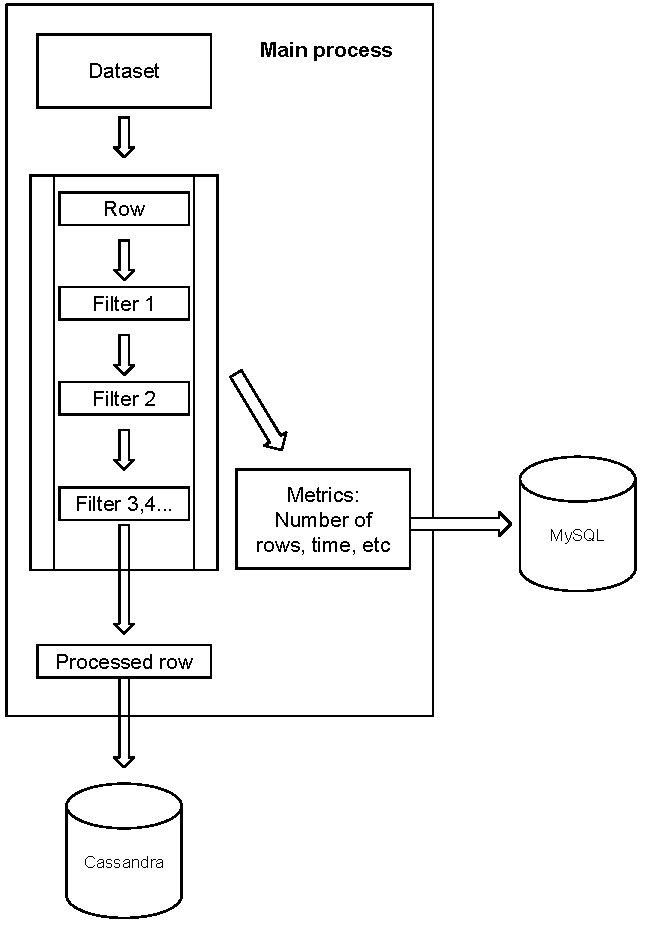
\includegraphics[width=120mm]{figures/program_overview_sequential.pdf}
  \caption[Sequential program overview.]{Sequential program overview.}
  \label{fig:sequential_program_overview}
\end{figure}

\chapter{Implementation}
    \section{Analysis of filter parallelizability}
Since the filters specify what the processing program should do to each row in a dataset, ``row by row'' or possibly chunks of rows is a suitable
granularity when implementing the parallelization of the program. Consequently, the filters of a file format are the prime candidates
for parallelization analysis. The analysis made is similar to the methodology used to identify the span in the work-span model described in
section \ref{work-span}. When applying the model to the problem of analyzing filters, a task is the processing of one row. In order to find
the tasks that need to be completed before other tasks, the filters that result in state that is accessed by subsequent rows or otherwise
affect the total processing of the dataset need to be identified.

Examining the filters, it is apparent that \textit{Dataset translation}, \textit{NullTranslationFilter}, \textit{Relation currency},
\textit{ThirdPartyAutomapper}, \textit{Set value}, \textit{RegExp extract}, and \textit{RegExp replace} only operate on the current dataset row, with no side effects.
This means that they produce no state changes that affect subsequent rows, which means that they do not affect the parallelizability of a dataset.

Additionally, \textit{Dataset information}, \textit{Tradefile information}, \textit{Temporary variable}, \textit{Logger}, and \textit{Skip row} perform
operations that either pull information from resources that are available to all rows, or produce an effect that does not affect any other rows.
The \textit{Conditional block} filter only produces effects according to its subfilters (a set of the filters already mentioned), and does not affect parallelization by itself.
\\\\
Hence, the filters that can affect the parallelization of a dataset are:
\begin{itemize}
  \item \textit{Mapping}, since the trade id mapping may need to keep track of state that can be accessed in subsequent rows in order to make all id:s unique.
  \item \textit{Header detection}, since all rows beneath the (first) header row depend on the column names for mappings and other values.
  \item \textit{Global variable}, since the variable may be written and accessed by any subsequent rows. Each rewrite of the variable needs to happen before the next rewrite,
    in the original, sequential order if the verification result is to be correct.
  \item \textit{State variable}, for the same reasons as Global variable.
  \item \textit{Stop processing}, if one thread sees a conditional fulfilled and stops processing, it is possible for another thread to keep processing rows that are intended
    to be ignored, thereby violating the constraints.
\end{itemize}



\section{Code inspection}
After an initial code and file format inspection, the following conclusions where made:
\begin{itemize}
  \item The \textit{Header detection} filter is effectively performed only once, as it is ignored for all rows after the one where the header was found.
  \item The filters \textit{Global variable} and \textit{State variable} make the processing of every row depend on the previous, as the writing of the variables may happen on each row.
  \item The process of making an ID unique could possibly be broken out to a post processing step.
  \item All file formats contain \textit{Header detection}, and many contain the make unique feature of the trade ID mapping.
  \item There are many file formats that do not have either \textit{Global variable}, \textit{State variable} or \textit{Stop processing} among their filters.
\end{itemize}

The conclusions above indicate that header detection may be done before creating the parallel processes, sending this data to each process when they are created.
If the process of producing unique ID:s is then done as a post processing step, the following task DAGs illustrate how the dependencies when processing different
file formats appear: In figure \ref{fig:embarrassing_dag}, the task DAG for a file format without a Global variable or State variable filter is illustrated.
In figure \ref{fig:embarrassing_dag}, the task DAG for a file format containing a Global variable is illustrated. Since the span is equal to the work
in the file formats containing Global variables or State variables, parallelization of datasets with these formats will result in no speedup according to the %Illustrate work-span?
work-span model (as $T_1 \leq T_\infty \Rightarrow S \leq 1$). File formats containing \textit{Stop processing} make it unfeasible to produce correct verification results
when parallelizing. Determination of whether the result is correct is non-viable if any rows are processed in different processes (as rows that should not be included in the result may be included anyway).

\begin{figure}[ht]
  \centering
  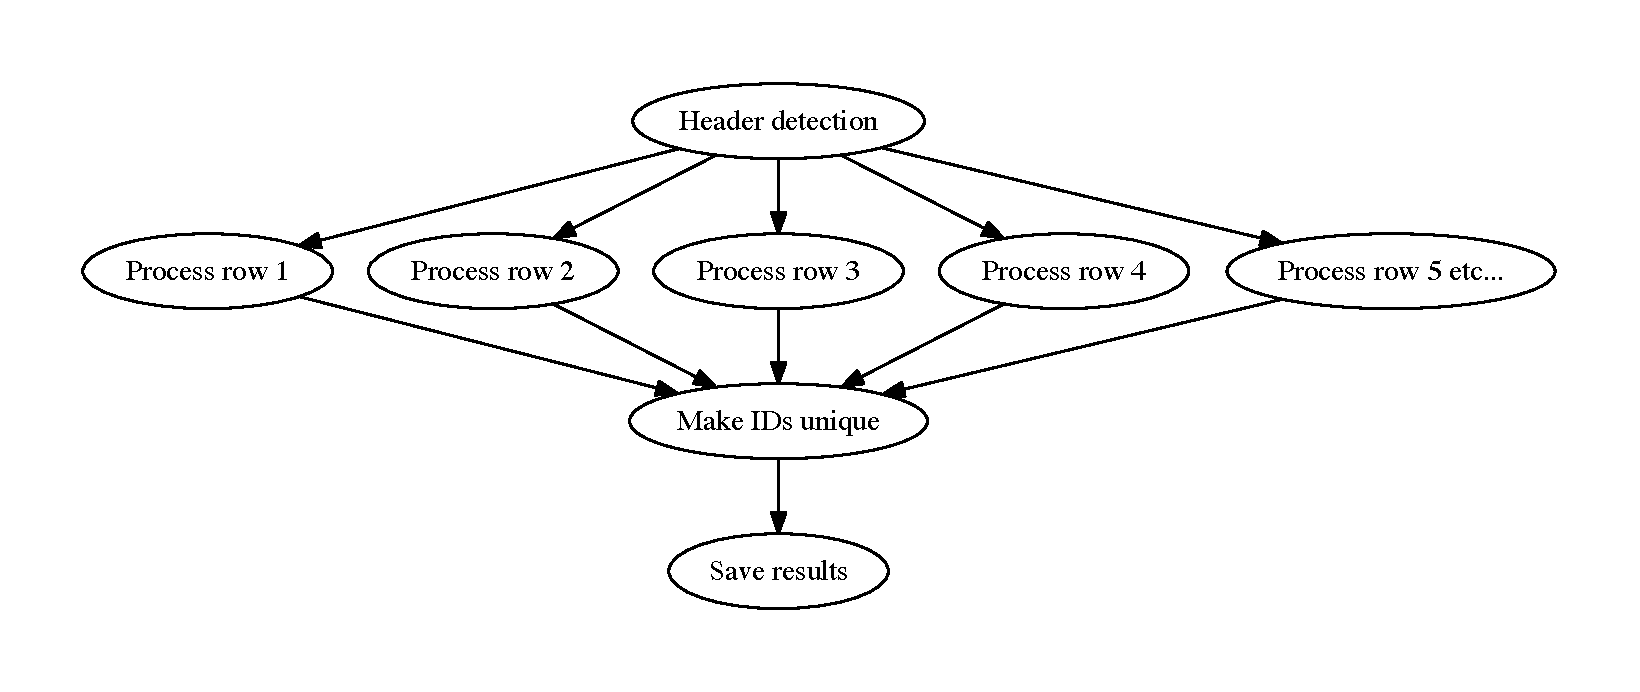
\includegraphics[width=120mm]{figures/embarrassing_file_format.pdf}
  \caption[Task DAG for a file format that does not contain global or state variables.]{An example of a task DAG for a file format that does not contain global variable or state variables. Header detections needs
  to be performed up front, and making trade IDs unique needs to be performed in a post processing step. The processing of each row does not depend on each other.}
  \label{fig:embarrassing_dag}
\end{figure}

\begin{figure}[ht]
  \centering
  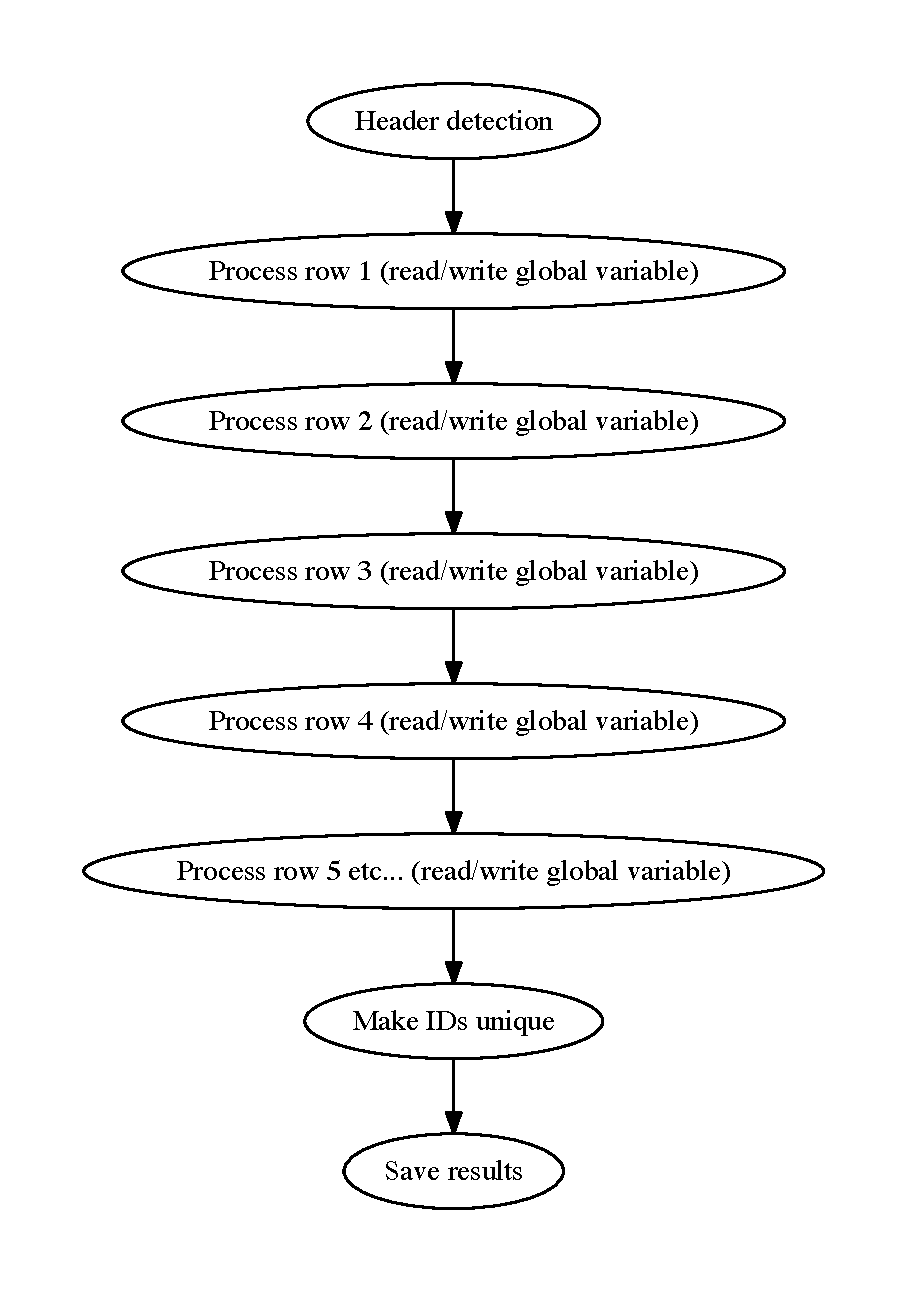
\includegraphics[width=120mm]{figures/global_variable_file_format.pdf}
  \caption[Task DAG for a file format that contains global or state variables.]{An example of a task DAG for a file format that contains global or state variables. Since each row may read and
  write the global (or state) variable, every task depends on the previous task.}
  \label{fig:global_dag}
\end{figure}

\section{Filter families}
With the help of the findings from the previous sections, families of filters with different characteristics can be identified.

\begin{itemize}
\item \textbf{Embarrassingly parallel filters} \\\\
The filters that do not affect parallelization in any way are:
\textit{Dataset translation}, \textit{NullTranslationFilter}, \textit{Relation currency},
\textit{ThirdPartyAutomapper}, \textit{Set value}, \textit{RegExp extract}, \textit{RegExp replace},
\textit{Dataset information}, \textit{Tradefile information}, \textit{Temporary variable}, \textit{Logger}, \textit{Skip row}, and \textit{Conditional block}.
In addition \textit{Mapping} is included among these filters if the make unique feature is disabled.
\item \textbf{Inherently serial filters} \\\\
The filters that enforce serial execution of the entire transformation are: \textit{Global variable}, \textit{State variable}, and \textit{Stop processing}.
\item \textbf{Overhead filters} \\\\ 
Filters that introduce parallelization overhead are: \textit{Mapping} (if the make unique feature is enabled) and \textit{Header detection}.
\end{itemize}

\section{File format families}
In addition to the filter families, the fact that the \textit{Header detection} filter is present in all file formats makes it possible to identify the following
file format families relevant to this thesis:

\begin{itemize}
\item \textbf{Embarrassingly parallel file formats} \\\\
  File formats that with the exception of \textit{Header detection} contain only embarrassingly parallel filters. 
\item \textbf{Extra overhead file formats} \\\\
  Formats that in addition to \textit{Header detection} and a number of embarrassingly parallel filters also contain \textit{Mapping} with the make unique filter enabled.
\item \textbf{Inherently serial file formats} \\\\
  Formats that contain any of the inherently serial filters.
\end{itemize}

\section{Parallelization} %TODO: skriv om ordning i dataset
In accordance with section \ref{related_work}, the Python \code{multiprocessing} module was used to implement the parallelization of the program. Additionally, measures where taken to send as little
data as possible between processes and to avoid introducing excessive complexity to the codebase. The \code{multiprocessing.Queue} facility was chosen for communication between processes due to its
noted performance and built-in synchronization \cite{singh_2013_parallel_padpwprfmm}.

Before deciding to use the parallelized version of program, the list of filters in a file format is examined for \textit{Global variable}, \textit{State variable}, or \textit{Stop processing}. If any of these are found, the
program falls back to its sequential version. Otherwise, the program carries on in accordance with figure \ref{fig:embarrassing_dag}. First, before creating any additional processes, the Header detection filter
is applied row by row until it produces a result (commonly after a few rows). Next, a (tunable) number of processes, as well as two queues are created. A number of row spans, or chunks, are then created by splitting
the rows beneath the header row into equally sized partitions. The first queue is used to transfer the data needed to process a chunk of the dataset, including the header data, the row span, and the result metadata.
In order to avoid errors and sending large objects between processes, only the primary key used to retrieve the result metadata object from the MySQL database is sent to the processes.
After this, the processes can independently retrieve the data. The second queue is used for sending the partial metrics objects for each chunk, and for indicating if a process is done processing
its data or if it encountered an error. Since all other results are written to the Cassandra database, this is the only information that needs to be sent to the main process. The queues can be
denoted the 'chunk queue' and the 'message queue', respectively.

In each of the created processes, the rows in the chunk are retrieved from the Cassandra database and a new object containing metrics for the chunk is created. The chunk is then processed as in the sequential program,
applying all filters to each row. The metrics object is updated during the processing, as in the original program. If the chunk was processed correctly, the metrics object is put on the message queue. Otherwise,
if an exception occurs, an error message is put on the queue instead. When all data in a process has finished processing, a message indicating that the process has finished its work is put on the message queue.

The main process continuously polls the message queue, and merges the partial metrics objects as they are polled from the queue. If an error message is encountered, an exception is raised on the main thread, mimicking the
behavior of the original sequential program. It also increments a counter whenever a done message is received from a process. When the counter is equal to the number of subprocesses, the main process stops waiting
for messages, and progresses with the post processing step of making the trade ID:s unique. Finally, the main process saves the result object with the corresponding merged metrics to the MySQL database. At this point,
the program has produced a finished verification result.

\section{Sources of overhead}
During the implementation of the parallel version of the program, the following possible sources of parallelization overhead where identified:

\begin{itemize}
  \item The \code{multiprocessing} module, where creating processes and transferring data between processes is costly.
  \item Less effective caching. Since the mappings cache is local to each subprocess, caches are built up individually. This results in fewer cache hits than in the sequential program, and more total work
    looking up values in the MySQL database.
  \item The process of making trade ID:s unique is added as an extra step after the main data processing pipeline.
  \item Because they lack built-in support for multiprocessing, the Python connections between both MySQL and Cassandra need to be restarted in the startup of each subprocess.
\end{itemize}

\chapter{Results}
    \section{Parallel program profiler analysis}
After the parallel program implementation, another round of profiling using \code{cProfile} was conducted. This was done on the initial testing laptop,
with 4 workers, on the same dataset as the first round of profiling. The results from the main process that orchestrates the other processes and aggregates their results can be
found in \ref{fig:parallel_profiler_main}. The results from two of the workers can be found in figure \ref{fig:parallel_profiler_w1} and figure \ref{fig:parallel_profiler_w2}.

For the main process, it is apparent that \code{post\_process\_parallel}, the function that makes the trade ID:s unique after the parallel worker processes have finished
executing, adds non-negligible overhead. \code{aggregate\_result} contains the code that creates the other processes and waits for these to produce their partial results,
aggregating them as they are produced. This code takes up 84\% of the total time, while the remaining 16\% of the code is effectively overhead.
In addtion, as mentioned in section \ref{section:sequential_profiler} as a possibility, \code{\_prepare} is called for each
worker process, resulting in extra overhead. It is conceivable that these sources of overhead are less noticable when processing a larger dataset, as the effects of
the functions that are called only one time take up a smaller amount of the total running time if the dataset contains a larger number of rows.

For the worker processes, the results are similar to the results from profiling the sequential program in section \ref{section:sequential_profiler}, but with lower
\code{cumtime} values. This is expected due to the lower number of rows per worker. The same functions as in the sequential program are responsible for the largest
portion of the running time, \code{process\_record}, \code{post\_process\_record}, \code{consume\_record}, and \code{\_prepare}.

\begin{figure}[ht]
  \lstinputlisting[basicstyle=\tiny]{figures/profiling_parallel_19_may_main.txt}
  \caption{Main process in parallel program \code{cProfile} output}
  \label{fig:parallel_profiler_main}
\end{figure}
\clearpage

\begin{figure}[ht]
  \lstinputlisting[basicstyle=\tiny]{figures/profiling_parallel_19_may_31147.txt}
  \caption{Worker 1 in parallel program \code{cProfile} output}
  \label{fig:parallel_profiler_w1}
\end{figure}
\clearpage

\begin{figure}[ht]
  \lstinputlisting[basicstyle=\tiny]{figures/profiling_parallel_19_may_31148.txt}
  \caption{Worker 2 in parallel program \code{cProfile} output}
  \label{fig:parallel_profiler_w2}
\end{figure}
\clearpage

\section{Transformation benchmarks}
The benchmarks for the experiments are outlined below. For each dataset, the results consist of a table containing
speedup, real time, user time, system time, and memory usage for each worker number. The standard deviation is represented
as a value following the $\pm$ sign. The value S in worker column signifies the original sequential program, while 1 is the
parallel program with a single worker. In addition to the tables, the real time, speedup, and memory usage are illustrated
using plots in order to visually demonstrate how the values change with the number of workers. In the plots for real time
and memory usage, the standard deviation is illustrated using black bars above and below each data point\footnote{
The standard deviation is shown for all plots of real time and memory usage, but it may be too small to be seen for some of the plots.}.

\section{Dataset 1}
The results for dataset 1 can be found in figures \ref{fig:dataset_1_table}, \ref{fig:dataset_1_real_time}, \ref{fig:dataset_1_speedup}, and \ref{fig:dataset_1_memory}.

\begin{figure}[ht]
\centering
\resizebox{\linewidth}{!}{%
\begin{tabular}{|c|c|c|c|c|c|}%
  \hline
  \bfseries Workers & \bfseries Speedup & \bfseries Real (s) & \bfseries User (s) & \bfseries System (s) & \bfseries Memory usage (MB)
  \csvreader[respect all,head to column names]{figures/dataset_1/dataset_1_table.csv}{workers=\w,speedup=\spd,real=\r,user=\u,system=\s,memory_usage_mb=\m}
  {\\\hline \w & \spd & \r & \u & \s & \m}
  \\ \hline
\end{tabular}}
\caption[Dataset 1 benchmark table.]{Dataset 1 benchmark table. The table displays the number of workers, the speedup (sequential run real time divided by real time), real time,
user time, system time, and memory usage. The standard deviation is displayed with a value following the $\pm$ sign.}
\label{fig:dataset_1_table}
\end{figure}

\begin{figure}[ht]
  \centering
  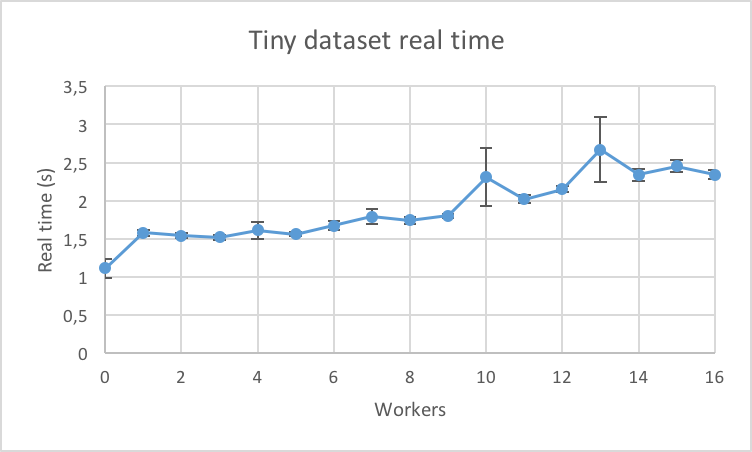
\includegraphics[width=120mm]{figures/dataset_1/dataset_1_real_time.png}
  \caption[Real time plot for dataset 1.]{Real time plot for dataset 1. The X axis shows the number of workers, where 0 signifies the sequential program run.
  The Y axis shows the real execution time for each worker value. The standard deviation is displayed with black bars around each data point. Real time
  increases as number of workers increase. The data points at 10 and 13 workers show high standard deviation.}
  \label{fig:dataset_1_real_time}
\end{figure}

\begin{figure}[ht]
  \centering
  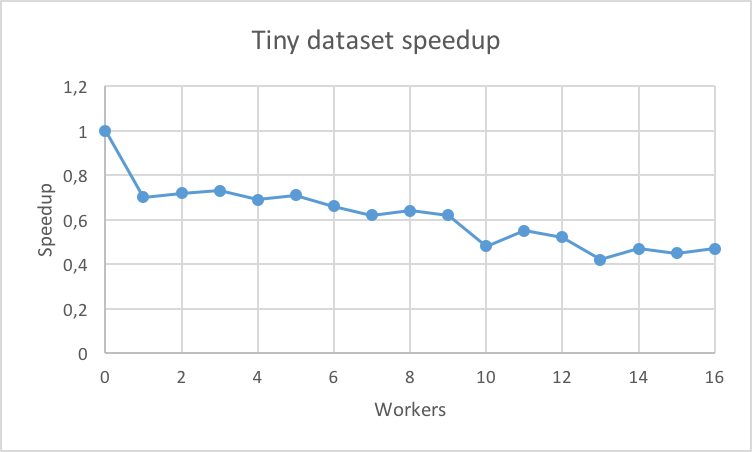
\includegraphics[width=120mm]{figures/dataset_1/dataset_1_speedup.png}
  \caption[Speedup plot for dataset 1.]{Speedup plot for dataset 1. The X axis shows the number of workers, and the Y axis shows a scalar value signifying the speedup as
  ``number of times faster than sequential execution''. Speedup decreases with each added worker, down to about half the speed of the sequential execution.}
  \label{fig:dataset_1_speedup}
\end{figure}

\begin{figure}[ht]
  \centering
  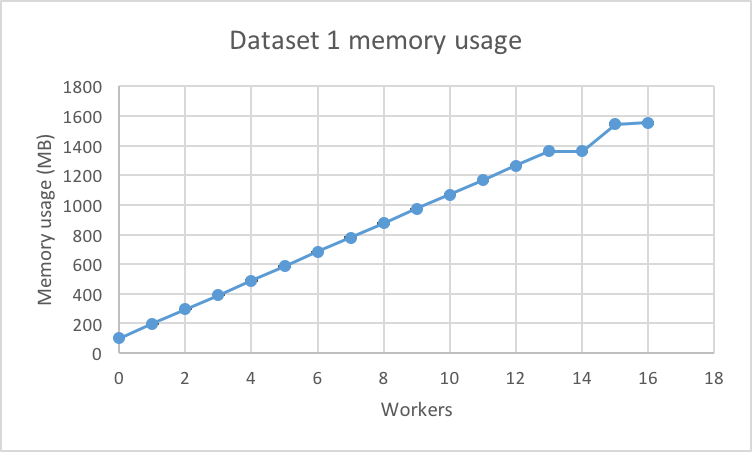
\includegraphics[width=120mm]{figures/dataset_1/dataset_1_memory.png}
  \caption[Memory usage plot for dataset 1.]{Memory usage plot for dataset 1. The X axis shows the numner of workers, and the Y axis shows the total memory usage as
  a sum of the highest memory usage for each worker process, in addition to the main process. Memory usage increases close to linearly with each added worker,
  up to about 1.6 GB for 16 workers.}
  \label{fig:dataset_1_memory}
\end{figure}

\section{Dataset 2}
The results for dataset 2 can be found in figures \ref{fig:dataset_2_table}, \ref{fig:dataset_2_real_time}, \ref{fig:dataset_2_speedup}, and \ref{fig:dataset_2_memory}.

\begin{figure}[ht]
\centering
\resizebox{\linewidth}{!}{%
\begin{tabular}{|c|c|c|c|c|c|}%
  \hline
  \bfseries Workers & \bfseries Speedup & \bfseries Real (s) & \bfseries User (s) & \bfseries System (s) & \bfseries Memory usage (MB)
  \csvreader[respect all,head to column names]{figures/dataset_2/dataset_2_table.csv}{workers=\w,speedup=\spd,real=\r,user=\u,system=\s,memory_usage_mb=\m}
  {\\\hline \w & \spd & \r & \u & \s & \m}
  \\ \hline
\end{tabular}}
\caption[Dataset 2 benchmark table.]{Dataset 2 benchmark table. The table displays the number of workers, the speedup (sequential run real time divided by real time), real time,
user time, system time, and memory usage. The standard deviation is displayed with a value following the $\pm$ sign.}
\label{fig:dataset_2_table}
\end{figure}

\begin{figure}[ht]
  \centering
  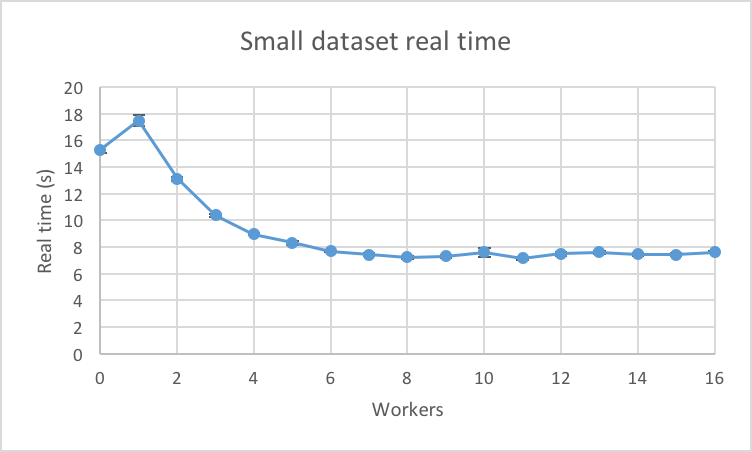
\includegraphics[width=120mm]{figures/dataset_2/dataset_2_real_time.png}
  \caption[Real time plot for dataset 2.]{Real time plot for dataset 2. The X axis shows the number of workers, where 0 signifies the sequential program run.
  The Y axis shows the real execution time for each worker value. The standard deviation is displayed with black bars around each data point. The real time
  decreases with each added worker up to 8 workers, where it evens out. The decrease in real time for each added worker becomes smaller as the number increases.}
  \label{fig:dataset_2_real_time}
\end{figure}

\begin{figure}[ht]
  \centering
  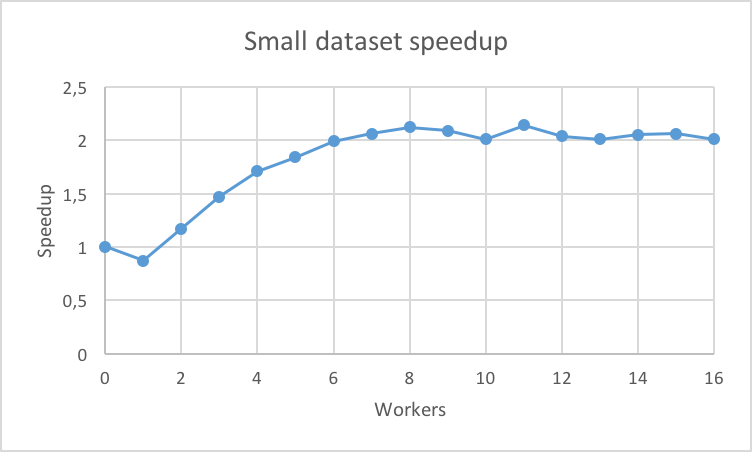
\includegraphics[width=120mm]{figures/dataset_2/dataset_2_speedup.png}
  \caption[Speedup plot for dataset 2.]{Speedup plot for dataset 2. The X axis shows the number of workers, and the Y axis shows a scalar value signifying the speedup as
  ``number of times faster than sequential execution''. Speedup increases with each worker, evening out around 8 workers and 2.1X speedup.}
  \label{fig:dataset_2_speedup}
\end{figure}

\begin{figure}[ht]
  \centering
  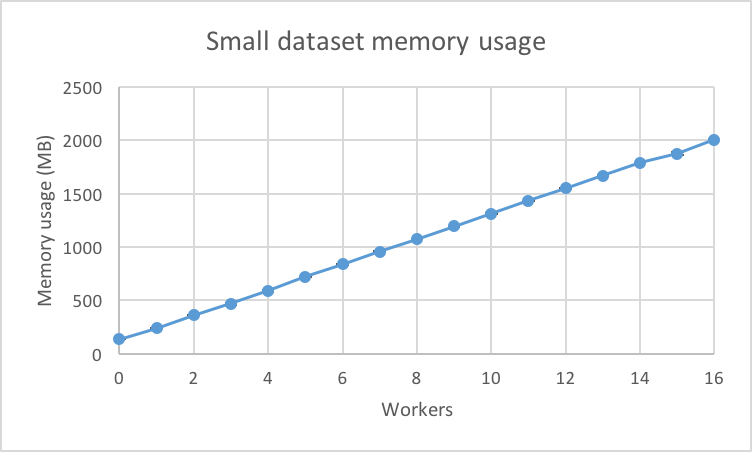
\includegraphics[width=120mm]{figures/dataset_2/dataset_2_memory.png}
  \caption[Memory usage plot for dataset 2.]{Memory usage plot for dataset 2. The X axis shows the numner of workers, and the Y axis shows the total memory usage as
  a sum of the highest memory usage for each worker process, in addition to the main process. Memory usage increases close to linearly with each added worker,
  up to about 2 GB for 16 workers.}
  \label{fig:dataset_2_memory}
\end{figure}

\section{Dataset 3}
The results for dataset 3 can be found in figures \ref{fig:dataset_3_table}, \ref{fig:dataset_3_real_time}, \ref{fig:dataset_3_speedup}, and \ref{fig:dataset_3_memory}.

\begin{figure}[ht]
\centering
\resizebox{\linewidth}{!}{%
\begin{tabular}{|c|c|c|c|c|c|}%
  \hline
  \bfseries Workers & \bfseries Speedup & \bfseries Real (s) & \bfseries User (s) & \bfseries System (s) & \bfseries Memory usage (MB)
  \csvreader[respect all,head to column names]{figures/dataset_3/dataset_3_table.csv}{workers=\w,speedup=\spd,real=\r,user=\u,system=\s,memory_usage_mb=\m}
  {\\\hline \w & \spd & \r & \u & \s & \m}
  \\ \hline
\end{tabular}}
\caption[Dataset 3 benchmark table.]{Dataset 3 benchmark table. The table displays the number of workers, the speedup (sequential run real time divided by real time), real time,
user time, system time, and memory usage. The standard deviation is displayed with a value following the $\pm$ sign.}
\label{fig:dataset_3_table}
\end{figure}

\begin{figure}[ht]
  \centering
  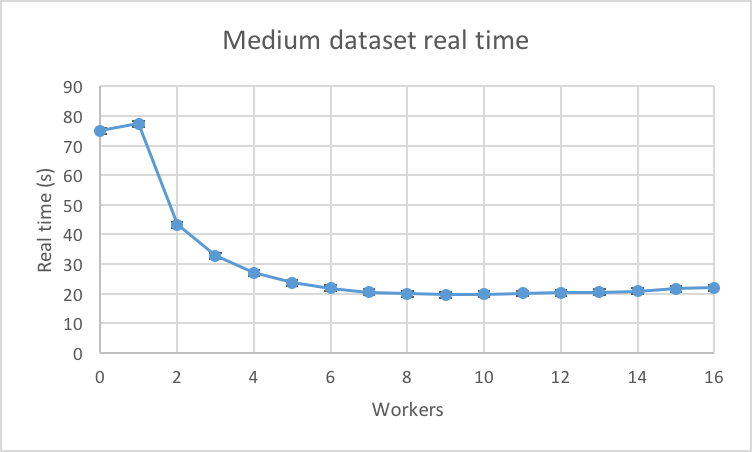
\includegraphics[width=120mm]{figures/dataset_3/dataset_3_real_time.png}
  \caption[Real time plot for dataset 3.]{Real time plot for dataset 3. The X axis shows the number of workers, where 0 signifies the sequential program run.
  The Y axis shows the real execution time for each worker value. The standard deviation is displayed with black bars around each data point. The real time
  decreases with each added worker up to 8 workers, where it evens out. The decrease in real time for each added worker becomes smaller as the number increases.}
  \label{fig:dataset_3_real_time}
\end{figure}

\begin{figure}[ht]
  \centering
  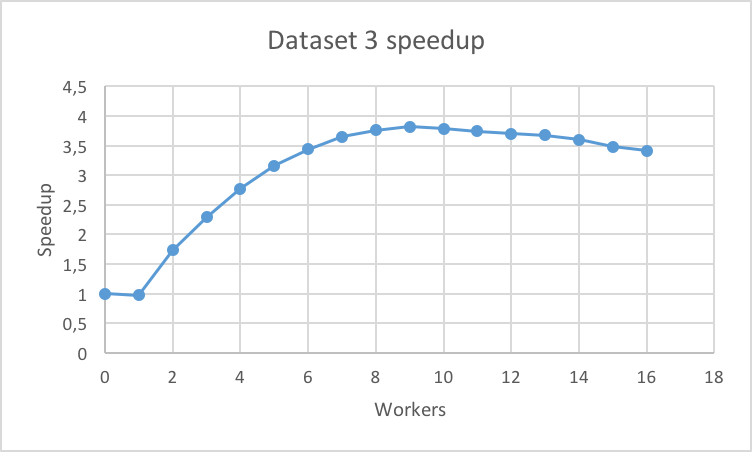
\includegraphics[width=120mm]{figures/dataset_3/dataset_3_speedup.png}
  \caption[Speedup plot for dataset 3.]{Speedup plot for dataset 3. The X axis shows the number of workers, and the Y axis shows a scalar value signifying the speedup as
  ``number of times faster than sequential execution''. Speedup increases with each worker, evening out around 8-9 workers and 3.8X speedup.}
  \label{fig:dataset_3_speedup}
\end{figure}

\begin{figure}[ht]
  \centering
  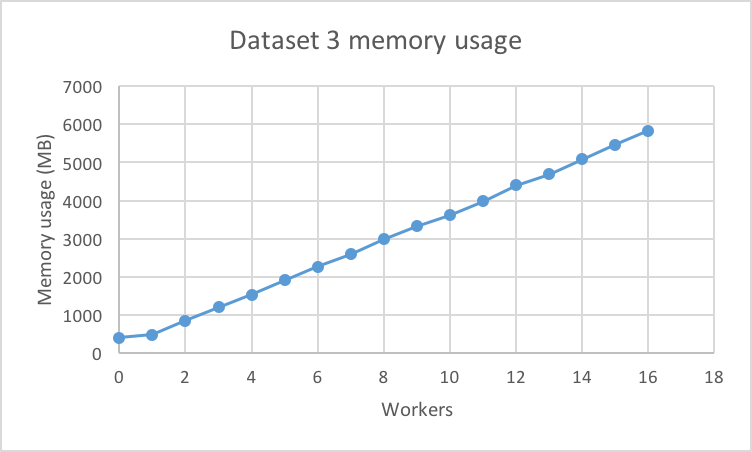
\includegraphics[width=120mm]{figures/dataset_3/dataset_3_memory.png}
  \caption[Memory usage plot for dataset 3.]{Memory usage plot for dataset 3. The X axis shows the numner of workers, and the Y axis shows the total memory usage as
  a sum of the highest memory usage for each worker process, in addition to the main process. Memory usage increases close to linearly with each added worker,
  up to about 6 GB for 16 workers.}
  \label{fig:dataset_3_memory}
\end{figure}


\section{Dataset 4}
The results for dataset 4 can be found in figures \ref{fig:dataset_4_table}, \ref{fig:dataset_4_real_time}, \ref{fig:dataset_4_speedup}, and \ref{fig:dataset_4_memory}.

\begin{figure}[ht]
\centering
\resizebox{\linewidth}{!}{%
\begin{tabular}{|c|c|c|c|c|c|}%
  \hline
  \bfseries Workers & \bfseries Speedup & \bfseries Real (s) & \bfseries User (s) & \bfseries System (s) & \bfseries Memory usage (MB)
  \csvreader[respect all,head to column names]{figures/dataset_4/dataset_4_table.csv}{workers=\w,speedup=\spd,real=\r,user=\u,system=\s,memory_usage_mb=\m}
  {\\\hline \w & \spd & \r & \u & \s & \m}
  \\ \hline
\end{tabular}}
\caption[Dataset 4 benchmark table.]{Dataset 4 benchmark table. The table displays the number of workers, the speedup (sequential run real time divided by real time), real time,
user time, system time, and memory usage. The standard deviation is displayed with a value following the $\pm$ sign.}
\label{fig:dataset_4_table}
\end{figure}

\begin{figure}[ht]
  \centering
  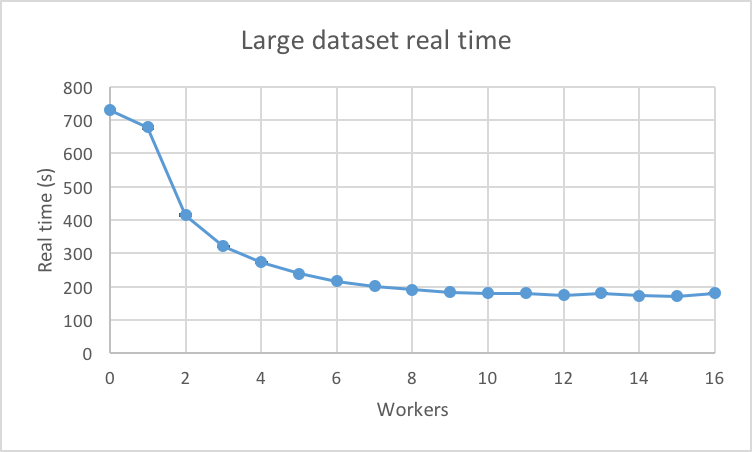
\includegraphics[width=120mm]{figures/dataset_4/dataset_4_real_time.png}
  \caption[Real time plot for dataset 4.]{Real time plot for dataset 4. The X axis shows the number of workers, where 0 signifies the sequential program run.
  The Y axis shows the real execution time for each worker value. The standard deviation is displayed with black bars around each data point. The real time
  decreases with each added worker up to 12 workers, where it evens out. The decrease in real time for each added worker becomes smaller as the number increases.}
  \label{fig:dataset_4_real_time}
\end{figure}

\begin{figure}[ht]
  \centering
  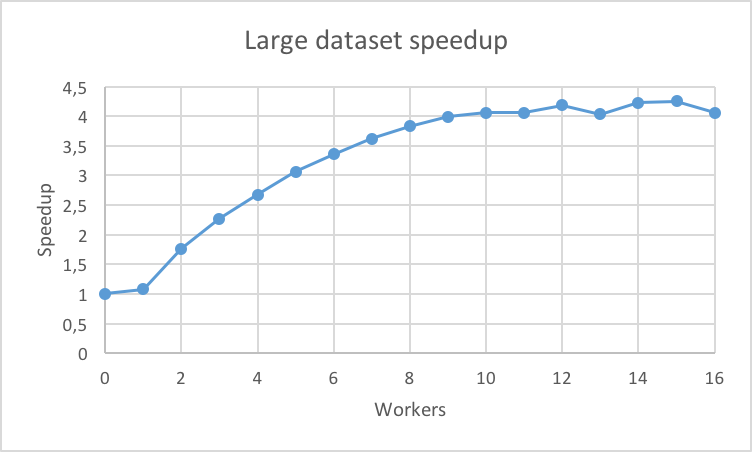
\includegraphics[width=120mm]{figures/dataset_4/dataset_4_speedup.png}
  \caption[Speedup plot for dataset 4.]{Speedup plot for dataset 4. The X axis shows the number of workers, and the Y axis shows a scalar value signifying the speedup as
  ``number of times faster than sequential execution''. Speedup increases with each worker, evening out around 12 workers and 4.2X speedup.}
  \label{fig:dataset_4_speedup}
\end{figure}

\begin{figure}[ht]
  \centering
  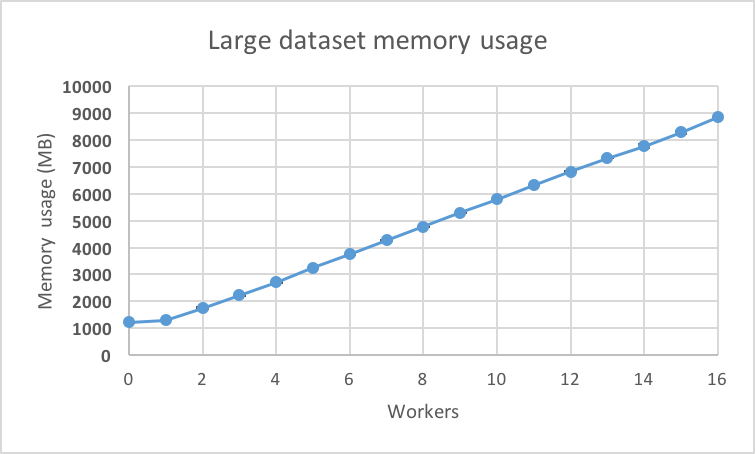
\includegraphics[width=120mm]{figures/dataset_4/dataset_4_memory.png}
  \caption[Memory usage plot for dataset 4.]{Memory usage plot for dataset 4. The X axis shows the numner of workers, and the Y axis shows the total memory usage as
  a sum of the highest memory usage for each worker process, in addition to the main process. Memory usage increases close to linearly with each added worker,
  up to about 8.8 GB for 16 workers.}
  \label{fig:dataset_4_memory}
\end{figure}


\chapter{Discussion}
    A discussion.
    
\nocite{*}
\printbibliography

%\appendix
\addappheadtotoc
%\chapter{RDF}\label{appA}


%\begin{figure}[ht]
%\begin{center}
%And here is a figure
%\caption{\small{Several statements describing the same resource.}}\label{RDF_4}
%\end{center}
%\end{figure}

%that we refer to here: \ref{RDF_4}

\end{document}
